\section{Extended Network Scenario}
In this section we will show how to extend the simple network topology (see
Section \ref{sec:SimpleNetworkScenario}). We will explain the additional
possibilities of building and configuring the extended network scenario:

The simple network topology is placed in the \emph{office-canvas} while the
additional elements are placed in the \emph{roadwarrior-canvas}. The
\emph{roadwarrior-canvas} consists of a router (\emph{roadwarrior-router}), a
PC (\emph{roadwarrior}) and a physical interface. The \emph{roadwarrior-router}
is connected to the \emph{office-router} on the \emph{office-canvas} through
the 192.168.3.0/24 network, the PC is in the 161.53.19.0/24 network whereas the
physical interface is in the 161.53.20.0/24 network.

We will now extend the simple network from the last chapter by adding the
\emph{roadwarrior-router}, \emph{roadwarrior} and the physical interface all
placed on another canvas. To open an existing IMUNES network configuration file
use \emph{File $\to$ Open} from the menubar or start IMUNES with the imn file
as an argument: \texttt{imunes simple-topology.imn}. Check that you are in the
edit mode. If not, switch with \emph{Experiment $\to$ Terminate}.

\subsection{Canvas Management}
To facilitate building of complex and large network topologies IMUNES lets you
divide the network topology into a set of network layers. These network layers
are called canvases.

Canvas management consists of two main elements:
\begin{itemize}
    \item Canvas menu in the menubar (Figure \ref{fig:canvas_menu})
    \item List of canvas tabs at the bottom of the main window, above the
statusbar (Figure \ref{fig:canvas_tabs_list})
    \begin{figure}[H]
	\centering
	\vspace{10pt}
	
\includegraphics[width=0.55\textwidth]{./images/canvas_tabs_list.png}
	\caption{\emph{Canvas Tabs}}
	\label{fig:canvas_tabs_list}
    \end{figure}
\end{itemize}

To add a new canvas use the \emph{Canvas $\to$ New} option from the menubar or
double click on the empty space in the canvas tabs list at the bottom of the
window.

You can rename the canvas with the \emph{Canvas $\to$ Rename} option from the
menubar or double click on the canvas tab in the canvas tabs list. (Figure
\ref{fig:canvas_rename}) Similarly the \emph{Canvas $\to$ Delete} option
deletes the active canvas.
\begin{figure}[H]
    \centering
    \vspace{10pt}
    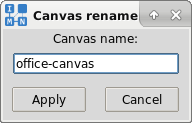
\includegraphics[width=0.25\textwidth]{./images/canvas_rename.png}
    \caption{\emph{Canvas rename dialog}}
    \label{fig:canvas_rename}
\end{figure}

There is also the option \emph{Canvas $\to$ Resize} that allows you to define a
custom canvas size in pixels. The default canvas size is 900*620 pixels.
(Figure \ref{fig:canvas_resize})
\begin{figure}[H]
    \centering
    \vspace{10pt}
    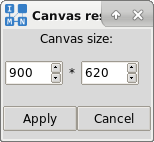
\includegraphics[width=0.20\textwidth]{./images/canvas_resize.png}
    \caption{\emph{Canvas resize dialog}}
    \label{fig:canvas_resize}
\end{figure}

Canvas selection can be done with the options from the \emph{Canvas} menu
(\emph{Previous, Next, First, Last}) or simply by clicking the tab with the
canvas name on it.

Rename the existing canvas \emph{Canvas0} into \emph{office-canvas}. Add a new
canvas, rename it into \emph{roadwarrior-canvas} and select it as the active
canvas. 

This canvas is empty so we will add a router by selecting the router tool and
clicking on the empty canvas. Rename this router into
\emph{roadwarrior-router}. Switch to the \emph{office-canvas}.  Now we will
connect the \emph{office-router} and the \emph{roadwarrior-router}. To do that,
right click on the \emph{office-router} and select \emph{Create link to $\to$
roadwarrior-canvas $\to$ roadwarrior-router} option (Figure
\ref{fig:create_link_to}) from the popped up menu. This will create a link
between \emph{roadwarrior-router} and \emph{office-router}.
\begin{figure}[H]
    \centering
    \vspace{10pt}
    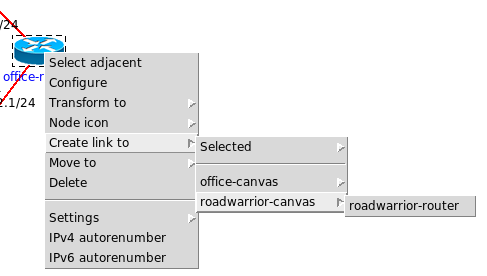
\includegraphics[width=0.65\textwidth]{./images/create_link_to.png}
    \caption{\emph{Create link to}}
    \label{fig:create_link_to}
\end{figure}

On the \emph{office-router} set the \emph{eth2} interface IPv4 address to
192.168.3.1/24. On the \emph{roadwarrior-router} set the \emph{eth0} interface
IPv4 address to 192.168.3.2/24.  We will add another PC to the
\emph{roadwarrior-canvas}, name it \emph{roadwarrior} and connect it with the
\emph{roadwarrior-router}. On the \emph{roadwarrior} set the eth0 IPv4 address
to 161.53.19.100/24. On the \emph{roadwarrior-router} set the eth1 IPv4 address
to 161.53.19.1/24.

The \emph{roadwarrior-router} uses the same dynamic routing model (quagga) as
the \emph{office-router} and we do not need to configure anything else on the
router. The \emph{roadwarrior} uses static routes and we will need to change
the default route gateway in static routes field of the \emph{roadwarrior}
configuration window to 0.0.0.0/0 161.53.19.1.

Finally, the configured network topology should look like the following (Figure
\ref{fig:office_canvas} and Figure \ref{fig:roadwarrior_canvas}):

\begin{figure}[H]
    \centering
%     \vspace{10pt}
    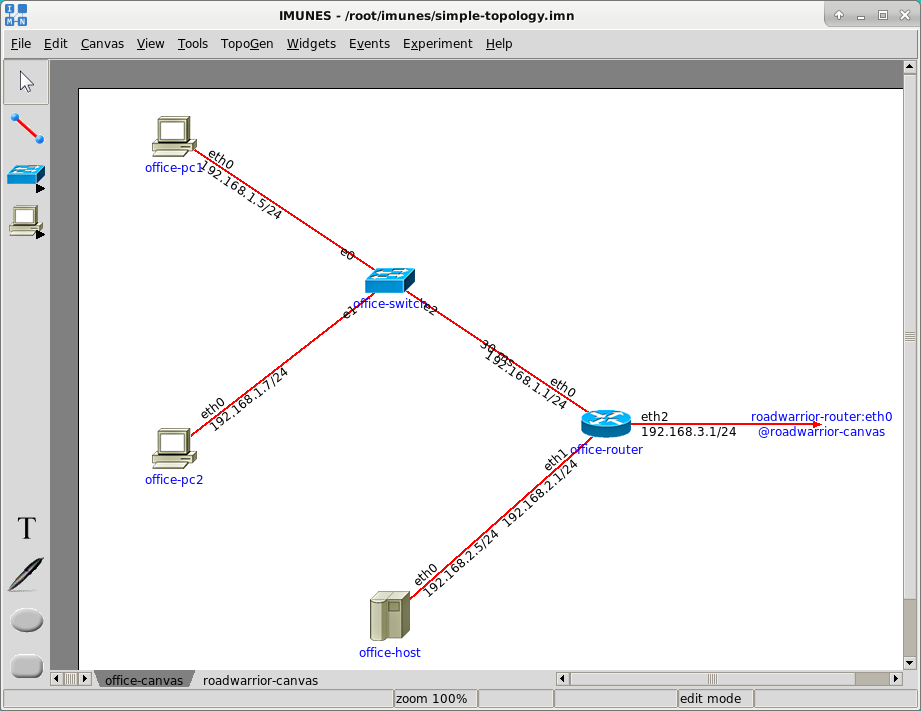
\includegraphics[width=\textwidth]{./images/office_canvas.png}
    \caption{\emph{office-canvas}}
    \label{fig:office_canvas}
\end{figure}

\begin{figure}[H]
    \centering
%     \vspace{10pt}
    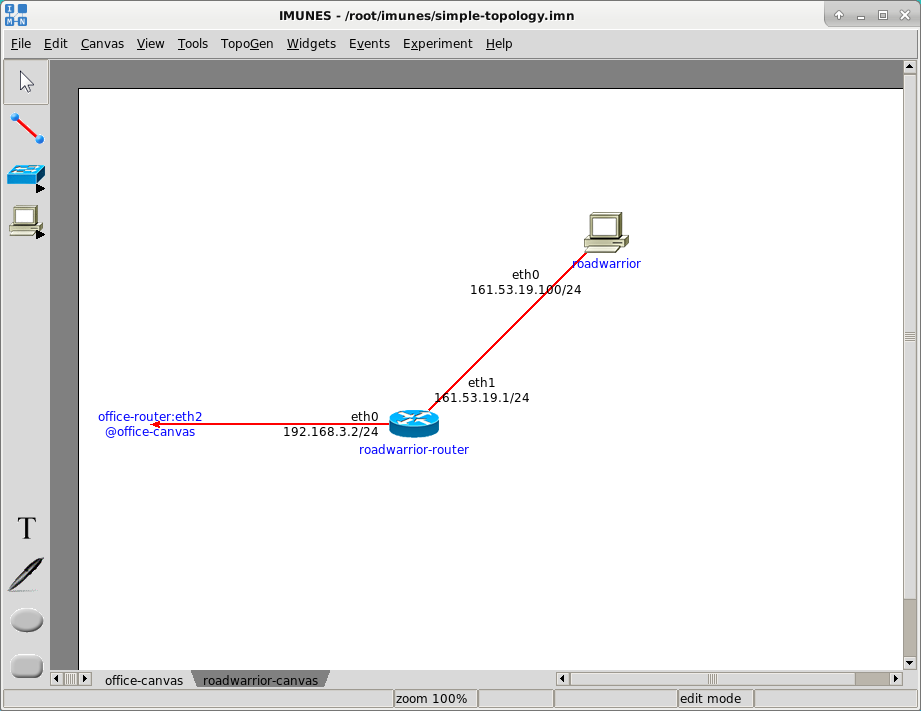
\includegraphics[width=\textwidth]{./images/roadwarrior_canvas.png}
    \caption{\emph{roadwarrior-canvas}}
    \label{fig:roadwarrior_canvas}
\end{figure}
 

Both the \emph{roadwarrior} and \emph{roadwarrior-router} can be easily moved
from \emph{roadwarrior-canvas} to \emph{office-canvas} with the \emph{Move To
$\to$ office-canvas} from the node menu. The link between
\emph{roadwarrior-router} and \emph{office-router}, as well as any other link,
can be deleted with the \emph{Delete} option from the \emph{Link} menu. To open
the \emph{link} menu, use the right click on the link and choose the
\emph{Delete} option.

When we are done with network configuration, we can start the experiment with
\emph{Experiment $\to$ Execute} from the menubar. We can now check that the
\emph{roadwarrior} can ping both networks (192.168.1.0/24, 192.168.2.0/24) and
additionally, that the network 192.168.1.0/24 does not have an access to the
\emph{roadwarrior}, but it has access to the 192.168.2.0/24 network.

\subsection{Attaching an external interface}

The \emph{External interface} tool from the toolbox provides the possibility to
attach a physical interface to a virtual node. This way the virtual network is
able to communicate with nodes from the external network.

We will now add the external interface to the \emph{roadwarrior-canvas}. To add
a external interface to the canvas select the \emph{External interface} tool
and click on the canvas.

\emph{External interface} nodes can be connected either with the LAN switch or the
router. Connect the newly created external interface with the virtual node
\emph{roadwarrior-router} using the \emph{Link} tool from the toolbox or the
\emph{Create link to} option from the node menu.

The newly created external interface node is unassigned and in the node name
field it contains \emph{UNASSIGNED}. Open the external interface configuration
window with a double click or right click on it and select the \emph{Configure}
option. Choose the name of the designated physical interface in the
\emph{Physical interface} drop-down list, e.g. em1, obtained from
\texttt{ifconfig -a} command ran on the physical machine (outside IMUNES).
(Figure \ref{fig:rj45_conf}) The name of the physical interface will appear in
the node name label. It is also possible to assign a VLAN tag to it. (Figure
\ref{fig:rj45_canvas})

\begin{figure}[H]
    \centering
%     \vspace{10pt}
    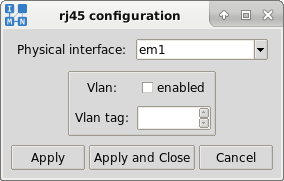
\includegraphics[width=0.37\textwidth]{./images/rj45_conf.png}
    \caption{\emph{External interface configuration dialog}}
    \label{fig:rj45_conf}
\end{figure}

\begin{figure}[H]
  \centering
  \vspace{10pt}
  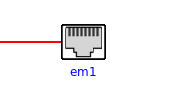
\includegraphics[width=0.15\textwidth]{./images/rj45_canvas.png}
  \caption{\emph{External interface node label}}
  \label{fig:rj45_canvas}
\end{figure}

Check that \emph{roadwarrior-router} has a properly configured IP address on
the network interface connected to the physical interface. Additionally, check
that routes which route packets between virtual network and the external
network through the physical interface exist in both the external network and
in the virtual network (on \emph{roadwarrior-router}).

Save this configuration to a new file by selecting the \emph{Save as} option
from the \emph{File} menu. Name the file \texttt{extended-topology.imn}.

\subsection{Attaching to a running experiment}
IMUNES gives you the possibility to run multiple independent experiments on one
physical computer. Therefore, we added the possibility of attaching to running
experiments through the IMUNES GUI. In the \emph{Experiment} menu, select the
option \emph{Attach to experiment}. A dialog similar to
\ref{fig:attach_to_experiment} is opened. Here you can select on which
experiment you would like to attach. You can attach to all experiments, those
that were started using batch mode and those that were executed from the GUI.
The window shows the following experiment parameters:

\begin{itemize}
\item Experiment ID
\item Filename of the topology
\item Time when the experiment was started.
\item Experiment screenshot (only if it was started through the GUI)
\end{itemize}

To attach to the you can double-click it's entry or use the \emph{Resume selected
experiment} button.
\begin{figure}[H]
  \centering
  \vspace{10pt}
  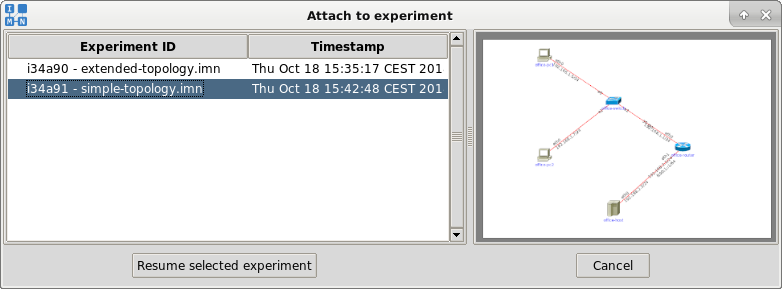
\includegraphics[width=0.90\textwidth]{./images/attach_to_experiment.png}
  \caption{\emph{Attach to experiment window}}
  \label{fig:attach_to_experiment}
\end{figure}
